\documentclass[twocolumn,english,notitlepage]{article}
\usepackage[margin=0.5in]{geometry}
\setlength{\parindent}{0pt} % no indents

% Math
\usepackage{amsmath}
\usepackage{physics}

% Citetations
\usepackage[ backend=bibtex, sorting=none, autocite=plain]{biblatex}
\addbibresource{refs/references}
\usepackage{xcolor}
\usepackage{hyperref}
\hypersetup{
    colorlinks,
    linkcolor={red!50!black},
    citecolor={blue!50!black},
    urlcolor={blue!80!black}}


% Formatting
\usepackage{float}
\usepackage{graphicx}
\graphicspath{ {./figs/} } 

% Misc
\usepackage{appendix}

% Commands

\title{Interesting title}
\author{Håkon Kvernmoen}
\date{MONTH YEAR}

\begin{document}
\maketitle

\section{Introduction}

\begin{figure}[H]
    \centering
    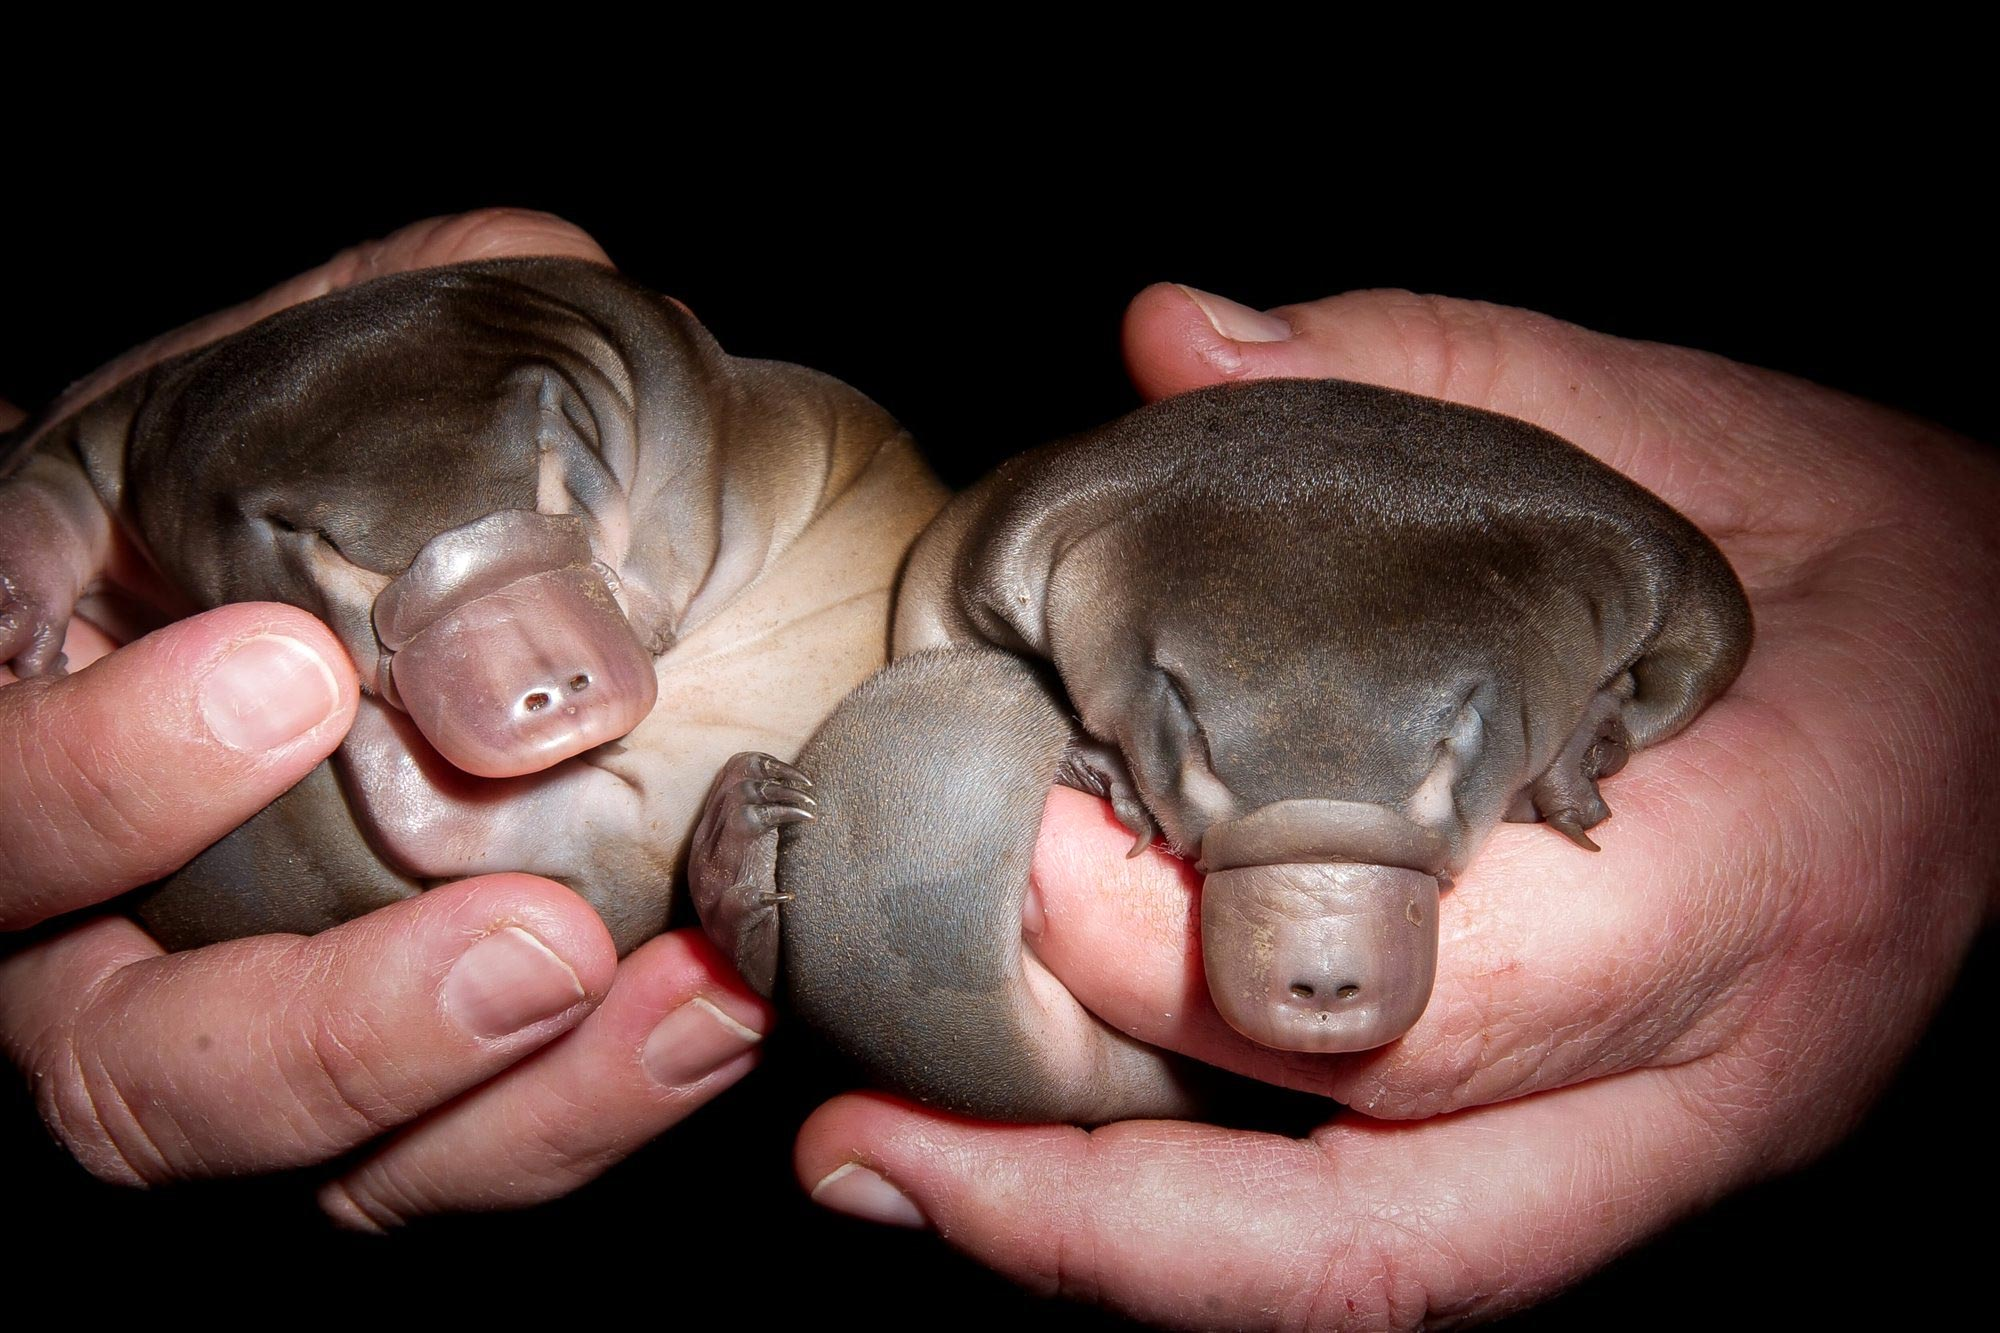
\includegraphics[width=0.5\linewidth]{Young-Platypus.jpg}
    \caption{Some figure caption}
    \label{fig:intro:plat}
\end{figure}

\section{Theory}
Example citation \cite{DFTgap}, example reference \eqref{eq:theo:curl}, example figure reference \ref{fig:intro:plat}

\begin{align}
	\int_{0}^{\infty} \dv{\Lambda}{\lambda} \dd{\lambda} = \Lambda(\infty) - \Lambda(0) \label{eq:theo:lambda}
\end{align}

\begin{align}
	\vb{A} = \curl{\vb{v}} \label{eq:theo:curl}  
\end{align}

\begin{appendix}
    \section{Appendix entry}
    some appendix things
\end{appendix}

\printbibliography

\end{document}

